\chapter{Background Theory and Motivation}\label{T-B}
\label{cha:TheoryAndBackground}

This project is a cross-disciplinary one, as it combines machine learning and medicine, and as such, some theory from both disciplines are necessary in order to understand the project.

\section{Background Theory}
\label{sec:no1}

\subsection{Lung Cancer}
\label{subsec:lung_cancer}

Lung cancer is the second most common type of cancer worldwide, and the the type of cancer with the highest total mortality worldwide, causing about 1.8 million deaths \citep{globalkreftforekomst}. Lung cancer is also the cancer type leading to the most deaths in Norway, amounting to 1500 deaths per year \citep{kreftnorge}. The most important risk factor related to lung cancer is smoking. Smoking is estimated to explain about 90\% of the risk of lung cancer in men, and 70\% to 80\% of the risk of lung cancer in women \citep{roykingrisiko}. Furthermore, about 90\% of lung cancer deaths in men, and 79\% of lung cancer deaths in women are caused by smoking \citep{roykingdod}.

There are two main types of lung cancer, Small Cell Lung Cancers (SCLC) and Non-Small Cell Lung Cancers (NSCLC) \citep{nsclcvsclc}. Of lung cancer cases, about 80-85\% are NSCLC, whilst 10-15\% of the cases are SCLC, and a few percent are non-mayor types of lung cancer \citep{nsclcvsclc2}. NSCLC cancers tend to grow slower than the SCLC cancer types, and thus SCLC has usually already spread when it is diagnosed \citep{nsclcvsclc2}. The NSCLC has three mayor subtypes, namely, adenocarcinoma (30-40\%), squamous cell (30\%) and large-cell undifferentiated carcinoma (10-15\%) \citep{nsclcvsclc}. The treatment and prognosis for the different NSCLC subtypes are similar \citep{nsclcvsclc2}.

Lung cancer develops in different stages. According to \citet{cancerstages}, the main four are:
\begin{enumerate}
    \item The cancer is only situated in your lung
    \item The cancer may have spread to the lymph nodes near the lung
    \item The cancer has spread deeper into the lymph nodes and into the middle of your chest
    \item Cancer is widespread throughout your body
\end{enumerate}

The main advantage with diagnosing lung cancer early is that the cancer has not yet spread to other parts of the body, which means that it can be removed by surgery \citep{cancertreatment}. On the other hand, later stages might require chemotherapy, radiation therapy or immunotherapy, but as the cancer has spread widely, this cure will likely not remove the cancer \citep{cancertreatment}.

%\citet{cancersurvival} found that the 5 year survival reat

\subsection{MicroRNA}

MicroRNA (miRNA) are short sequences of RNA, about 22 nucleotides each, that regulates the expression of mRNA by binding to the target mRNA sequence, and thus stopping it from being translated. Circulating miRNA has been found to be a biomarker for many diseases, including cancer, infectious diseases and mental illnesses \citep{mirnabiomarker,mirnabiomarker2,mirnabiomarker3,mirnabiomarker4}. miRNA-sequences are usually named with the prefix "miR-" and then a unique number that is incremented for each discovey of a miRNA-sequence. The most commonly used database with known miRNA-sequences is the miRBase database \citep{mirbase}.

\subsection{MicroRNA and Lung Cancer}

The overall role role of miRNA in relation to lung cancer is not fully understood \citep{mirnarole}. MicroRNA is thought to be both function as tumor suppressor genes and as oncogenes \citep{mirnarole2}. 

\subsection{MicroRNA profiling methods}

There are several methods for measuring levels of miRNA. The most common ones are qRT-PCR, microarrays and sequencing. Here is a very high level description of the different methods. For more technical details see e.g. \citet{mirnatech}. The different technologies typically have different issues.

\subsubsection{qRT-PCR}
Quantitative Reverse Transcription - Polymerase Chain Reaction (qRT-PCR) is the most common method in the studies used in this project. As the name implies, the process depend on reverse transcription, where miRNA are reverse transcripted, using the enzyme reverse transcriptase, into complementary DNA (cDNA). The results are then monitored using polymerase chain reactions.

In qRT-PCR, one needs a primer for each miRNA-sequence that should be measured. Therefore it can only measure miRNA-sequences that are decided beforehand. The main advantage of qRT-PCR is that it is the most sensitive method of the different technologies \citep{mirnatech}, which means that the results are more accurate, and that it also works well when the consentration of miRNA is low. 

\subsubsection{Microarrays}
Micoroarrays are what is called a hybridization method. It starts out similarly to qRT-PCR, with converting miRNA into cDNA, only that the miRNA in this case are fluorescently labled. The microarray has several spots, each with single-stranded DNA samples (called probes) that are mounted to the microarray. When the cDNA are added to the microarray, the cDNA will bind to the DNA samples that have the same sequence, in a process called hybridization. Afterwards, the microarray is washed clean, and only the cDNA that has managed to bind will remain. Thus, by checking for the fluorescence of the different spots, one can find which DNA-probes had cDNA bind to it, and which had not. The level of fluorescence can then be used as the concentration of the corresponding miRNA-sequence.

The main advantage of microarrays is that it is the cheapest of the main technologies \citep{mirnatech}. The disadvantages is that it has low sensitivity, and that you have to decide beforehand what miRNA-sequences you want to measure, as you need to populate the microarray with the corresponding DNA-probes.  

\subsubsection{Sequencing}
Sequencing also starts with converting miRNA into cDNA. A primer is then connected to the cDNA in one direction. The sequencing step works by adding fluorescent bases one by one, and then see if they adds to the sequence starting with the primer. Thus, one can read out the sequence of the cDNA.

The main disadvantage of sequencing is that it is expensive \citep{mirnatech}. It is also less sensitive than qRT-PCR. The main advantage, however, is that you do not need to decide beforehand the miRNA-sequences you want to measure.


\subsection{Variance stabilizing transformation}
\label{subsec:var_stab}

In miRNA measurements, one often see that the variance in miRNA concentration is a function of the mean miRNA concentration. One possible transformation is the log transformation where one takes the logarithm of the data. That can change a curve where $\text{Var}[y] \propto \text{E}[y]^2$ into a curve where the variance of $y$ is independent of the mean of $y$. One example of this can be seen in \autoref{fig:log_transformation}.

\begin{figure}
    \foreach \time in {Before, After}{
    \begin{subfigure}[b]{0.5\textwidth}
    \resizebox{\textwidth}{!}{
    \begin{tikzpicture}
    \begin{axis}[
        xlabel={Mean miRNA concentration},
        ylabel={Variance of miRNA concentration},
    ]
    \addplot[
        scatter,only marks,scatter src=x,
        table/col sep=comma,
        scatter/use mapped color={draw=blue, fill=blue}
    ]
    table[x=means,y=variances]{tables/VarianceStabilizing/\time.csv};
    \end{axis}
    \end{tikzpicture}
    }
    \caption{\time \ log transformation}
    \label{fig:log_transformation_\time}
    \end{subfigure}
    }
    \caption{Mean and variance in different miRNA sequences in \citep{Ma2011}}
    \label{fig:log_transformation}
\end{figure}

Another advantage of a variance stabilizing transformation is to ensure that the data is not skewed. Other statistical tools like explained variance (\autoref{subsec:explained_variance}) assumes that the underlying data has a normal distribution. A normal distribution, however have no skew, therefore unskewing the data is necessary for ensuring that other methods are giving valid results. More formally, if we assume that $Y ~ g(X)$ for some function $g$ and that $X \sim N(\mu, \sigma)$, then doing the transformation $y' = g^{-1}(y)$ ensures that our variables are normally distributed. In particular, if we assume that $g(X) = e^{X}$, then the log-transformation will ensure that our data is normally distributed. 

\subsection{Loess regression}
\label{subsec:loess_regression}

Loess regression is also sometimes called local regression, and it is a type of regression that is made for smooting scatterplots \citep{loess}. The regression works by fitting a low degree polynomial for each datapoint. The fitting of each polynomial works by giving weight to nearby points, where more weight is given to points near the original datapoint. The regression value for each datapoint is thus the value of the corresponding polynomial evaluated in this point.

Loess regression is practical when mean and variance still are not independent after a log transformation. Using loess regression can ensure that they become independent as shown in \autoref{fig:loess_regression}

\begin{figure}
    \foreach \time in {Before, After}{
    \begin{subfigure}[b]{0.5\textwidth}
    \resizebox{\textwidth}{!}{
    \begin{tikzpicture}
    \begin{axis}[
        xlabel={Mean miRNA concentration},
        ylabel={Variance of miRNA concentration},
    ]
    \addplot[
        scatter,only marks,scatter src=x,
        table/col sep=comma,
        scatter/use mapped color={draw=blue, fill=blue}
    ]
    table[x=means,y=variances]{tables/VarianceStabilizing/\time.csv};
    \end{axis}
    \end{tikzpicture}
    }
    \caption{\time \ log transformation}
    \label{fig:log_transformation_\time}
    \end{subfigure}
    }
    \caption{Mean and variance in different miRNA sequences in \citep{Ma2011}}
    \label{fig:log_transformation}
\end{figure}


\subsection{Principal component analysis}

Principal component analysis (PCA) is a method of data reduction, where a dataset in $\mathbb{R}^n$ is projected down on a lower dimensional vector space $\mathbb{R}^m$. The projection in PCA is the projection that ensures that the most of the variance of the original dataset is kept, whilst ensuring that the projection is not expanding the dataset. One of the main advantages of PCA is that you could project a dataset down to just two or three dimensions, which makes it possible to plot the dataset.

\subsection{Explained variance}
\label{subsec:explained_variance}

Explained is a way of analyzing the sources of variance in a dataset. Using linear regression, one assumes that the dependent variable $y$, covariates $\mathbf{X}$ and residuals $\epsilon \sim N(0, \sigma)$ have the relationship $y = \mathbf{X}\beta + \epsilon$, for some parameter vector $\beta$.


If one creates a linear regression model of the dataset one get a parameter vector $\hat{\beta}$ which is the maximum likelihood estimate of $\beta$, and predictions $\hat{y} = \mathbf{X} \hat{\beta}$ for $y$. Also define $\mathbf{SST} = \sum_i \left(y_i - \bar{y}\right)^2$ is the total sum of squares, $\mathbf{SSR} = \sum_i \left(\hat{y_i} - \bar{y}\right)^2$ is the sum of squares due to regression and $\mathbf{SSE} = \sum_i \left(y_i - \hat{y_i}\right)^2$ is the sum of squared estimate of errors. Then we have the following relationship:
$$\mathbf{SST} = \mathbf{SSR} + \mathbf{SSE}$$

The proportion of the empirical variance that can be explained by the covariates is thus
$$R^2 = \frac{\mathbf{SSR}}{\mathbf{SST}}$$

\subsection{Logistic regression}

Assume that you have Bernulli trials where each $y_i \sim \text{Bernoulli}(p_i)$ with the relationship:
$$\frac{p}{1-p} = e^{\mathbf{X}\beta}$$
for some covariates $\mathbf{X}$ and some parameter vector $\beta$.
Then one can show that
$$p = \frac{1}{1 + e^{-\mathbf{X}\beta}}$$
A logistic regression model can find $\hat{\beta}$, the maximum likelihood estimate of $\beta$.

Logistic regression is a relatively simple classification model, and in the studies used in this project, logistic regression is the most commonly used model for diagnosing lung cancer based on miRNA levels.


\subsection{XGBoost}

XGBoost is a machine learning algorithm that is based on gradient tree boosting \citep{xgboost}. Boosting algorithms are machine learning algorithms that combine weak models into stronger models, by using the combined output of several weak models. Gradient boosting is a type of boosting algorithm that uses an idea similar to gradient descent in order to find optimal weights given to each of the weaker models \citep{gradientboosting}. Instead of using the gradient directly, the algorithm just ensure that the weights are updated such that the loss function is lowered in each step. Gradient tree boosting is gradient boosting where the weak models are decision trees. XGBoost's decision trees have default directions of descending in the tree if there are missing data, thus good handling missing values is one of XGBoost's biggest advantages.

XGBoost is a popular machine learning algorithm on the machine learning contest site Kaggle\footnote{\url{https://www.kaggle.com}}, winning 17 of 29 contests in 2015 \citep{xgboost}.

\subsection{Miscellaneous statistical measures}

\subsubsection{Fold change}
Fold change is defined as the ratio of a certain value between two different populations. In this project, the fold change used is typically the ratio levels of a certain miRNA-sequence between cases and controls. % As most calculation in this project is done on log-transformed data, this ratio is the difference of levels.




\iffalse
The background theory depth and breadth depends on the depth needed to understand your project in the different disciplines that your project crosses.  It is not a place to just write about everything you know that is vaguely connected to your project. The theory is here to help the reader that does not know the theoretical basis of your work so that he/she can gain sufficient understanding to understand your contributions. In particular, the theory section provides an opportunity to introduce terminology that can later be used without disturbing the text with a definition.  In some cases it will be more appropriate to have a separate section for different theory. However, watch that you don't end up with too short sections. Subsections may also be used to separate different background theory. 

When introducing techniques or results, always reference the source. Be careful to reference the original contributor of a technique and not just someone who happens to use the technique. For relevant results to your work, you would want to look particularly at newer results so that you have referenced the most up-to-date work in your area. If you don't have the source handy when writing, mark the test that a reference is needed and add it later. 

Web pages are not reliable sources --- they might be there one day and removed the next; and thus should be avoided, if possible. A verbal discussion is not a source and should not be referenced or described in the text.  

The bulk of citations in the report will appear in section~\ref{cit}. However, you will often need to introduce some terminology and key citations already in this chapter. 

You can cite a paper in the following manners: 

\begin{itemize}
\item when referring to authors:\\
 \citet{authorson10:_secon_best_paper_in_world} stated something rather nice.
\item to cite indirectly: \\
 Papers should be written nicely \citep{authorson10:_secon_best_paper_in_world}\\
or\\
In \cite{authorson10:_secon_best_paper_in_world}, a less detailed template was presented.
\item To just cite the authors: \\
\citeauthor{authorson10:_secon_best_paper_in_world} wrote a nice paper.
%\item Or just the year: \citeyear{authorson10:_secon_best_paper_in_world}.
%\item You can even cite specific pages: \citet[p. 3]{authorson10:_secon_best_paper_in_world}.
\end{itemize}

\vspace{0.5cm}

\noindent
{\bf Introducing figures:} \\

\begin{figure}[ht]
\begin{center}
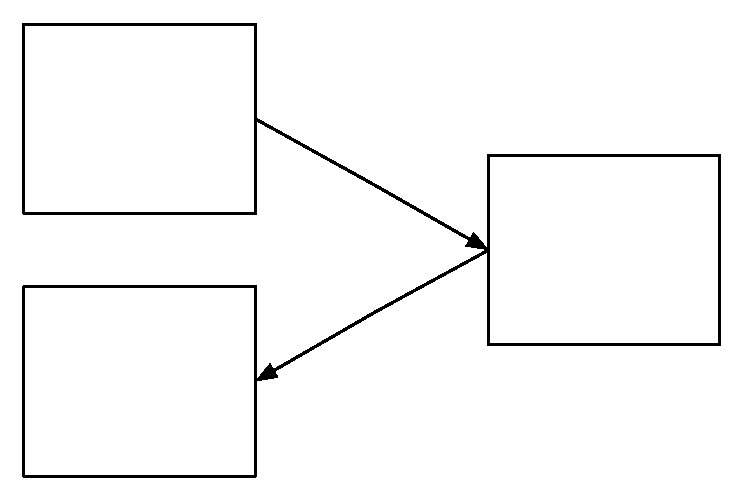
\includegraphics[width=0.5\columnwidth]{figs/figure1.pdf}
\caption[Boxes and arrows are nice]{Boxes and arrows are nice (adapted from \citet{authorson10:_secon_best_paper_in_world})}
\label{fig:BoxesAndArrowsAreNice}
\end{center}
\end{figure}

Remember that when you borrow figures you should always credit the original author --- such as Figure \ref{fig:BoxesAndArrowsAreNice} (adapted from \citet{authorson10:_secon_best_paper_in_world}). Also don't just put the figure in and leave it to the author to try to understand what the figure is. The figure should be put in to convey a message and you need to help the author to understand the message intended by explaining the figure in the text. 

\vspace{0.5cm}

\noindent
{\bf Introducing tables in the report: }\\

\begin{table}[htbp]
\begin{center}
\begin{tabular}{|c|c|c|c|c|}\hline\hline
This & is & a & nice & table\\\hline
This & is & a & nice & table\\\hline\hline
\end{tabular}
\caption{Example Table}
\end{center}
\label{tab:ExampleTable}
\end{table}%

As you can see from Table \ref{tab:ExampleTable}, tables are nice. However, again, you need to discuss the contents of the table in the text. You don't need to describe every entry but draw the authors attention to what is important for he/she to glean from the table. 
\fi

\section{Structured Literature Review Protocol}
\label{sec:literature_review}

The point of the literature search was to find studies relevant to miRNA and circulating lung cancer. The main search engine used was PubMed\footnote{\url{pubmed.ncbi.nlm.nih.gov/}}, which is a commonly used search engine for medical litterature. The search term used was:
\begin{verbatim}
(lung OR pulmonary OR NSCLC) and (tumor OR cancer OR carcinoma) and
(microRNA* OR miRNA* OR miR*) and (diagnosis OR biomarker OR detection)
and (serum or plasma or "whole blood")
\end{verbatim}
In addition, I search in databases that have public gene expression data as shown in \autoref{tab:genedatabase}.
\begin{table}[htbp]
\begin{center}
\begin{tabular}{|p{0.25\textwidth}|p{0.75\textwidth}|}\hline
Database name & Search term\\\hline
ArrayExpress\tablefootnote{\url{https://www.ebi.ac.uk/arrayexpress/}} & \verb|microrna lung cancer|\\\hline
Gene Expression Omnibus (GEO)\tablefootnote{\url{https://www.ncbi.nlm.nih.gov/gds}} & \verb|(mirna OR microrna) AND "lung cancer"| \verb|AND (diagnosis OR detection) |\\\hline
OmicsDI\tablefootnote{\url{https://www.omicsdi.org}} & \verb|"lung cancer" AND TAXONOMY: 9606 AND| \verb|-"breast cancer" AND (mirna OR microrna)| \verb|AND (serum OR plasma OR "whole blood")|\\\hline
\end{tabular}
\caption{Search in public gene expression databases}
\label{tab:genedatabase}
\end{center}
\end{table}

The inclusion criteria where based on what datasets I thought was relevant to this project:
\begin{itemize}
    \item The paper is an experiment where circulating miRNA is measured.
\end{itemize}
Some of the studies measured miRNA levels in the lung tissue or in sputum, rather than measuring circulating miRNA. As the values are somewhat different between lung tissue miRNA and circulating miRNA \citep{differentserumtissue}, only the circulating miRNA ones was selected in order to have a consistent dataset. In addition, the research question was to look at the diagnostic value of circulating miRNA, which makes it most reasonable to base on circulating miRNA data.

\begin{itemize}
    \item The study both have people diagnosed with lung cancer and controls not diagnosed with lung cancer.
\end{itemize}

The controls in some of the studies are not healthy, but suffers from other kind of lung diseases. Other studies have both have both healthy controls, and controls with other lung illnesses. Both are relevant, as on one hand, one would like to see the difference between healthy controls and patients with lung cancer in order to remove miRNA changes due to other illnesses. On the other hand, people who are getting checked for lung cancer often have lung issues, which is the reason for their checkup.

Some studies were excluded as they did not have a control group e.g. \citet{Mitchell2017}.

\begin{itemize}
    \item At least four different miRNA sequences were measured.
\end{itemize}

The point of this project is to combine and compare datasets. Having few miRNA sequences measured makes it hard to combine datasets, as there is a high likelihood that there are no overlapping miRNA sequences between the datasets. It is also hard to compare datasets measuring completely different miRNA sequences.

\begin{itemize}
    \item Meta-analyses were used as source of relevant studies
\end{itemize}

Some of the studies found were meta-analyses. In that case relevant studies were retrieved from the references of the meta-analysis.

\iffalse
Here you need to include your structured review protocol including search engine, search words, research questions  (for search, not the masters research questions), inclusion createrias and evaluation Criterias. 
\fi

\section{Motivation}
\label{sec:no2}

\iffalse
Your motivation can be either application driven or technique/methodology driven. However in both cases, there will be an element of methodology driven due to the research focus of our group and the nature of a masters project.  
What other research has been conducted in this area and how is it related to your work? The text should clearly illustrate why your goals and research questions are important to address. This section is thus where your literate review will be presented. It is important when presenting the review that you present an overview of the motivating elements of the work going on in your field and how these relate to your proposal, rather than a list of contributors and what they have done. This means that you need to extract the key important factors for your work and discuss how others have addressed each of these factors and what the advantages/disadvantages are with such approaches. As you mention other authors, you should reference their work. Note that the reference list reflects the literature you have read and have cited. This will only be a subset of the literature that you have read.
\fi
